\documentclass{beamer}

\usepackage{graphicx}
\usetheme{Szeged}
\usecolortheme{beaver}

\author{Anne Wanningen \and Xeryus Stokkel}
\title[Week 6]{Introduction to Computer Graphics Raytracer week 6}

\begin{document}

\maketitle

\section{Gooch Shading}

\begin{frame}
	\begin{columns}[T]
		\begin{column}{.3\textwidth}
			\begin{figure}
				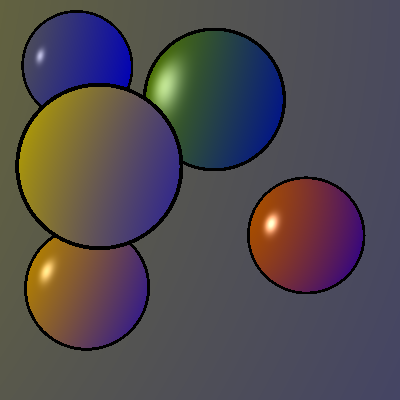
\includegraphics[width=\textwidth]{ref.png}
			\end{figure}
		\end{column}
		\begin{column}{.3\textwidth}
			\begin{figure}
				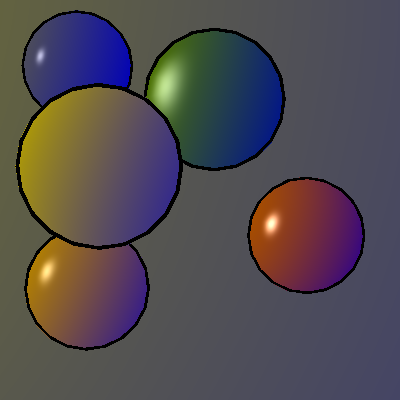
\includegraphics[width=\textwidth]{res.png}
			\end{figure}
		\end{column}
		\begin{column}{.3\textwidth}
			\begin{figure}
				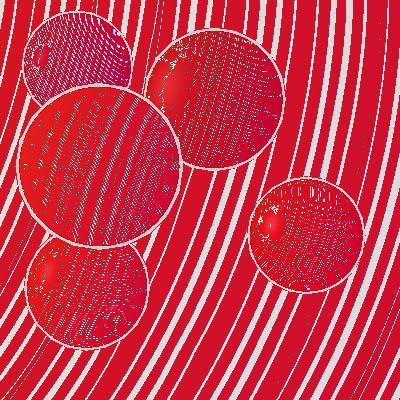
\includegraphics[width=\textwidth]{diff.png}
			\end{figure}
		\end{column}
\end{columns}
\end{frame}

\section{Texture mapping}
\begin{frame}
	\begin{columns}[T]
		\begin{column}{.45\textwidth}
			\begin{figure}
				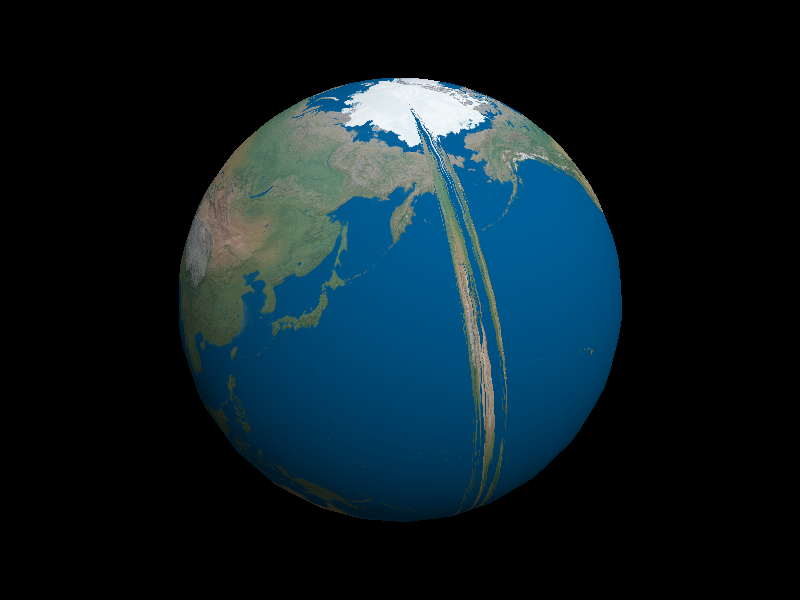
\includegraphics[width=\textwidth]{screen_2015-03-25_12:02:27}
			\end{figure}
		\end{column}
		\begin{column}{.45\textwidth}
			\begin{figure}
				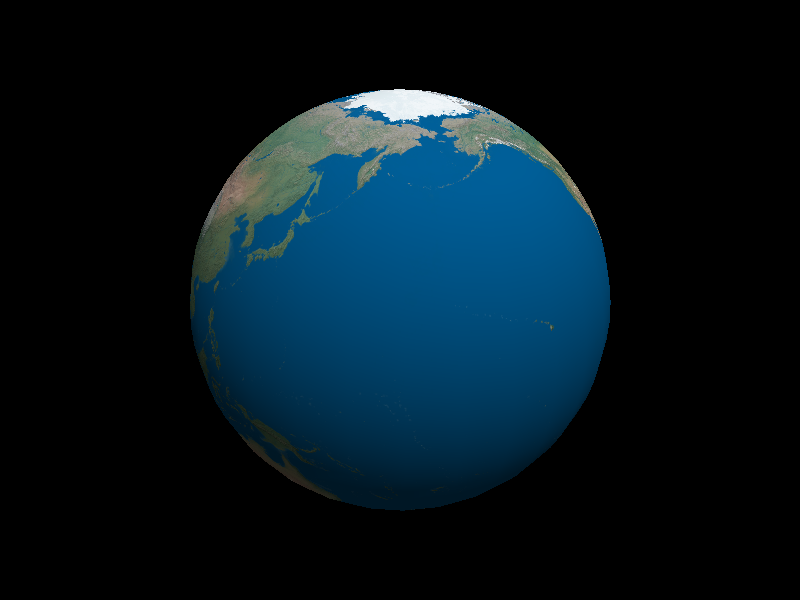
\includegraphics[width=\textwidth]{screen_2015-03-25_12:02:57}
			\end{figure}
		\end{column}
	\end{columns}
\end{frame}
\begin{frame}
	\begin{figure}
		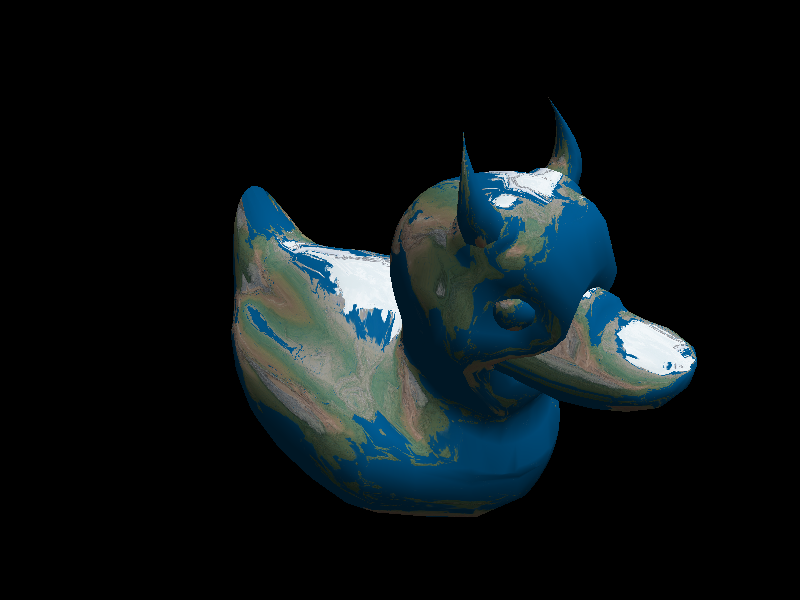
\includegraphics[height=.9\textheight]{screen_2015-03-25_12:10:25}
	\end{figure}
\end{frame}

\section{Animation}
\begin{frame}
	\begin{figure}
		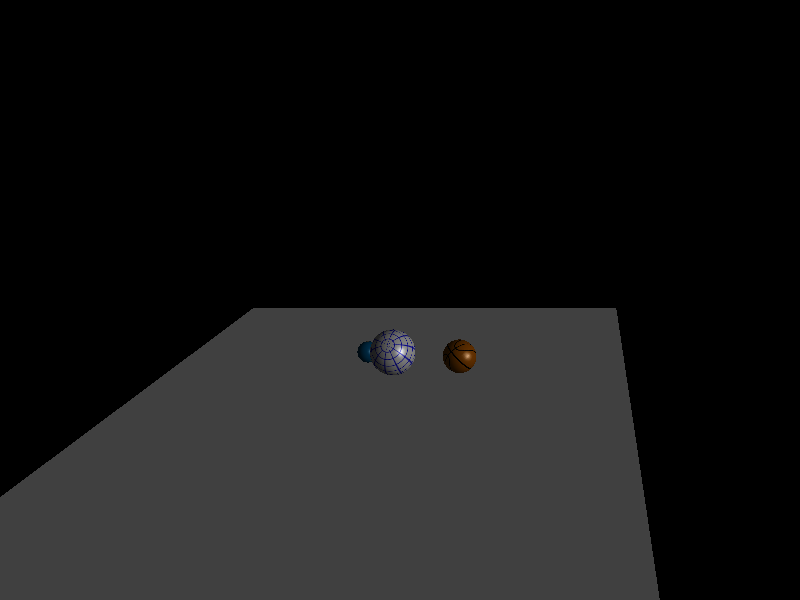
\includegraphics[height=.9\textheight]{screen_2015-03-25_12:04:03}
	\end{figure}
\end{frame}
\end{document}
